\documentclass[12pt]{article}
\usepackage[utf8]{inputenc}
\usepackage[spanish]{babel}
\usepackage{graphicx}
\usepackage{float}
\usepackage{amsmath}

\title{Proyecto Piloto\thanks{Proyecto piloto realizado con el fin de practicar los conocimientos adquiridos en el taller.}}
\author{Leonard David Vivas Dallos\thanks{Estudiante de Pregrado en Ciencias de la Computación de la Universidad Nacional de Colombia}}
\date{\today}

\begin{document}
\maketitle

\tableofcontents

\section{Introducción}
En el presente documento se manejarán los conceptos adquiridos en clase, haciendo la transcripción de un informe realizado en la aplicación Word, y presentado como parte de una actividad correspondiente a la materia de Cálculo Diferencial. El documento descrito fue escogido para este fin dado a que usa de manera precisa y conveniente la mayoría de los ítem en la presentación. Se verán el manejo de los siguientes conceptos.

\begin{itemize}
    \item Tipo de archivo.
    \item Notas al pie de página y agradecimientos.
    \item Índices.
    \item Secciones y subsecciones.
    \item Manejo de figuras y tablas.
    \item Tipo de letras.
    \item Listados.
    \item Escritura matemática.
\end{itemize}

\section{Informe Actividad 1 Tarea 4}
Tomando en cuenta el fractal conocido como \textit{Esponja de Menger}, pero en dos dimensiones, denotamos que podríamos estar analizando la \textit{Alfombra de Sierpinski}, ya que la \textit{Esponja} por definición es la generalización tridimensional de la \textit{Alfombra}, la cual es a su vez una generalización bidimensional del conjunto de Cantor.

\begin{figure}[H]
    \centering
    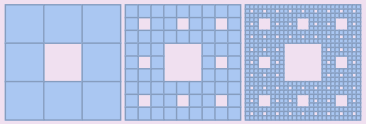
\includegraphics{Imágenes/Img_1.png}
    \caption{Paso 1,2,3 del fractal}
    \label{Img_1}
\end{figure}
\begin{figure}[H]
    \centering
    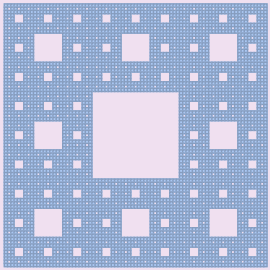
\includegraphics[width=5cm]{Imágenes/Img_2.png}
    \caption{Paso 4 del fractal}
    \label{Img_2}
\end{figure}

\subsection{Cálculo de la dimensión fractal D:}
Teniendo en cuenta la función $N(s)=s^{-D}$, y sabiendo que N corresponde al número de copias del objeto a escala ``s". Notemos que hay 8 copias del cuadrado, cada uno de un tercio de lado con respecto al original. Así, $N(s)=8$; $s=\frac{1}{3}$, reemplazando nos queda:

\begin{equation*}
    8=\left(\frac{1}{3}\right)^{-D}
\end{equation*}
\begin{equation*}
    D=\frac{log(8)}{log(3)}\cong1.892789261
\end{equation*}

Para saber la cantidad de cuadraditos blancos más pequeños que se ven en la figura del 4° paso, basta con usar la función $N(s)=s^{-D}$ para buscar cuantos cuadrados del estilo del 1° paso hay en el cuarto, esto ya que por cada cuadrado de este estilo tenemos 1 cuadradito blanco. Así pues, sabemos que cada una de estas copias mide $\frac{1}{27}$ de la longitud original. Como anteriormente hallamos la dimensión fractal, podemos usar estos datos para buscar $N(s)$

\begin{equation*}
    N(s)=s^{-D}
\end{equation*}
\begin{equation*}
    N(s)=\left(\frac{1}{27}\right)^{-1.892789261}\cong512.0000005
\end{equation*}

Como por cada copia tenemos 1 cuadradito blanco, podemos decir que en el cuarto paso tenemos 512 cuadraditos blancos, lo que corresponde al mismo valor si lo miramos gráficamente, o por la fórmula $8^3$, que corresponde a la cantidad de divisiones que se toman (8), con respecto a la cantidad de veces que se realiza el procedimiento (3).

\subsection{Perímetro, suponiendo que el lado de la esponja es 1}
Definamos el lado original de la esponja $l_0=1$, así sabemos que el perímetro original es $P_0=4$. Ahora bien, como por cada paso debemos suprimir 1 cuadrado de los 9 que formamos, a $P_0$ debemos sumarle el perímetro del cuadrado que hemos quitado, que correspondería a los bordes de la figura por dentro.

\subsubsection{Caso 1}
$n=1$\\
Sabemos que el lado de cada cuadrado formado en este paso el $l_1=\frac{1}{3}$. Con esto, tenemos que el perímetro en el primer paso es $P_1=P_0+4l_1$. Desarrollando:

\begin{equation*}
    P_1=P_0+4\left(\frac{1}{3}\right)
\end{equation*}
\begin{equation*}
    P_1=4+\frac{4}{3}=\frac{16}{3}\cong5.3
\end{equation*}

\subsubsection{Caso 2}
$n=2$\\
$l_2=\frac{1}{9}$. Para este caso, debemos adicionar al perímetro de la figura del anterior paso, el perímetro de los cubos formados en este paso, que son 8.

\begin{equation*}
    P_2=P_1+8\left(4\left(\frac{1}{9}\right)\right)
\end{equation*}
\begin{equation*}
    P_2=\frac{16}{3}+\frac{32}{9}=\frac{80}{9}\cong8.89
\end{equation*}

\subsubsection{Caso 3}
$n=3$\\
$l_3=\frac{1}{27}$

\begin{equation*}
    P_3=P_2+8\left(8\left(4\left(\frac{1}{27}\right)\right)\right)
\end{equation*}
\begin{equation*}
    P_3=\frac{80}{9}+\frac{256}{27}=\frac{496}{27}\cong18.370
\end{equation*}

\subsubsection{Caso 4}
$n=4$\\
$l_4=\frac{1}{81}$

\begin{equation*}
    P_4=P_3+8\left(8\left(8\left(4\left(\frac{1}{81}\right)\right)\right)\right)
\end{equation*}
\begin{equation*}
    P_4=\frac{496}{27}+\frac{2048}{81}=\frac{3536}{81}\cong43.65432099
\end{equation*}

Apliquemos la siguiente fórmula para los casos y encontremos que se mantiene la igualdad

\begin{equation}
    P(n)=4\left[1+\frac{1}{3}\sum_{k=0}^{n-1}\left(\frac{8}{3}\right)^k\right]
\end{equation}
\begin{equation*}
    P(1)=4\left[1+\frac{1}{3}*\left(\frac{8}{3}\right)^0\right]=4\left(1+\frac{1}{3}\right)=4*\frac{4}{3}=\frac{16}{3}
\end{equation*}
\begin{equation*}
    P(2)=4\left[1+\frac{1}{3}*\left\{\left(\frac{8}{3}\right)^0+\left(\frac{8}{3}\right)^1\right\}\right]=4\left[1+\frac{1}{3}\left(1+\frac{8}{3}\right)\right]
\end{equation*}
\begin{equation*}
    =4\left[1+\frac{1}{3}*\frac{11}{3}\right]=4\left[1+\frac{11}{9}\right]=4\left[\frac{20}{9}\right]=\frac{80}{9}
\end{equation*}
\begin{equation*}
    P(3)=4\left[1+\frac{1}{3}*\left\{\left(\frac{8}{3}\right)^0+\left(\frac{8}{3}\right)^1+\left(\frac{8}{3}\right)^2\right\}\right]=4\left[1+\frac{1}{3}\left\{1+\frac{8}{3}+\frac{64}{9}\right\}\right]
\end{equation*}
\begin{equation*}
    =4\left[1+\frac{1}{3}*\frac{97}{9}\right]=4\left[1+\frac{97}{27}\right]=4\left[\frac{124}{27}\right]=\frac{496}{27}
\end{equation*}
\begin{equation*}
    P(4)=4\left[1+\frac{1}{3}*\left\{\left(\frac{8}{3}\right)^0+\left(\frac{8}{3}\right)^1+\left(\frac{8}{3}\right)^2+\left(\frac{8}{3}\right)^3\right\}\right]
\end{equation*}
\begin{equation*}
    =4\left[1+\frac{1}{3}\left\{1+\frac{8}{3}+\frac{64}{9}+\frac{512}{27}\right\}\right]=4\left[1+\frac{1}{3}*\frac{803}{27}\right]
\end{equation*}
\begin{equation*}
    =4\left[1+\frac{803}{81}\right]=4\left[\frac{884}{81}\right]=\frac{3536}{81}
\end{equation*}

Partamos de la fórmula ya usada, demostremos que $P(n)=\frac{16}{15}\left[3+2\left(\frac{8}{3}\right)^{n-1}\right]$ y veamos que pasa cuando n tiende a infinito. Para iniciar, simplifiquemos la suma geométrica aparte:

\begin{equation*}
    \frac{1}{3}\sum_{k=0}^{n-1}\left(\frac{8}{3}\right)^k=\frac{1}{3}\left(\frac{1-\left(\frac{8}{3}\right)^n}{1-\frac{8}{3}}\right)=\frac{1}{3}\left(\frac{1-\left(\frac{8}{3}\right)^n}{-\frac{5}{3}}\right)=\frac{1}{3}\left(\frac{-3}{5}\right)\left(1-\left(\frac{8}{3}\right)^n\right)
\end{equation*}
\begin{equation*}
    =\frac{-3}{15}\left(1-\left(\frac{8}{3}\right)^n\right)
\end{equation*}

Teniendo esta respuesta, remplacemos en la fórmula inicial:

\begin{equation*}
    P(n)=4\left[1+\frac{-3}{15}\left(1-\left(\frac{8}{3}\right)^n\right)\right]
\end{equation*}
\begin{equation*}
    =4\left[1+\left(-\frac{3}{15}+\frac{3}{15}\left(\frac{8}{3}\right)^n\right)\right]=4\left[1+\frac{1}{15}\left(-3+3\left(\frac{8}{3}\right)^n\right)\right]
\end{equation*}
\begin{equation*}
    =4+\frac{4}{15}\left(-3+3\left(\frac{8}{3}\right)^n\right)=4-\frac{12}{15}+\frac{12}{15}\left(\frac{8}{3}\right)^n=4\left[1-\frac{3}{15}+\frac{3}{15}\left(\frac{8}{3}\right)^n\right]
\end{equation*}
\begin{equation*}
    =\frac{3}{3}*4\left[1-\frac{3}{15}+\frac{3}{15}\left(\frac{8}{3}\right)^n\right]=\frac{4}{3}\left[3-\frac{9}{15}+\frac{9}{15}\left(\frac{8}{3}\right)^n\right]=\frac{4}{3}\left[3-\frac{3}{5}+\frac{3}{5}\left(\frac{8}{3}\right)^n\right]
\end{equation*}
\begin{equation*}
    =\frac{4}{3}\left[\frac{15-3}{5}+\frac{3}{5}\left(\frac{8}{3}\right)^n\right]=\frac{4}{3}\left[\frac{12}{5}+\frac{3}{5}\left(\frac{8}{3}\right)^n\right]=\frac{4}{3}*\frac{1}{5}\left[12+3\left(\frac{8}{3}\right)^n\right]
\end{equation*}
\begin{equation*}
    =\frac{4}{15}\left[12+3\left(\frac{8}{3}\right)^n\right]=\frac{4}{15}\left[12+3*\left(\frac{8}{3}\right)\left(\frac{8}{3}\right)^{n-1}\right]=\frac{4}{15}\left[12+\frac{24}{3}\left(\frac{8}{3}\right)^{n-1}\right]
\end{equation*}
\begin{equation*}
    =\frac{4}{15}\left[12+8\left(\frac{8}{3}\right)^{n-1}\right]=\frac{4}{15}\left[4\left(3+2\left(\frac{8}{3}\right)^{n-1}\right)\right]=\frac{16}{15}\left(3+2\left(\frac{8}{3}\right)^{n-1}\right)
\end{equation*}

Intuitivamente, tal como se referenció, a medida que aumenta n, aumenta el perímetro de la función (esponja). Es decir, cuando $n\rightarrow\infty, P(n)\rightarrow\infty$
\end{document}